\documentclass[tikz,border=10pt]{standalone}
\usetikzlibrary{arrows.meta}

\tikzset{
    vertex/.style={circle, fill=black, inner sep=2pt},
    edge/.style={thick, -Stealth},
    removable edge/.style={dashed, thick, -Stealth}
}

\begin{document}
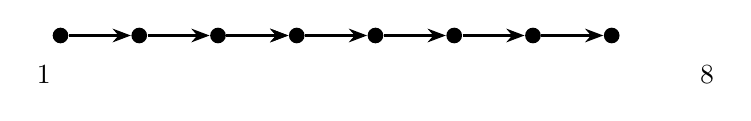
\begin{tikzpicture}[scale=1]

% Vertices
\node (v1) at (0,0) [vertex] {};
\node (v2) at (1,0) [vertex] {};
\node (v3) at (2,0) [vertex] {};
\node (v4) at (3,0) [vertex] {};
\node (v5) at (4,0) [vertex] {};
\node (v6) at (5,0) [vertex] {};
\node (v7) at (6,0) [vertex] {};
\node (v8) at (7,0) [vertex] {};

% Edges
\draw[edge] (v1) -- (v2);
\draw[edge] (v2) -- (v3);
\draw[edge] (v3) -- (v4);
\draw[edge] (v4) -- (v5);
\draw[edge] (v5) -- (v6);
\draw[edge] (v6) -- (v7);
\draw[edge] (v7) -- (v8);

% Removable edge
\draw[removable edge] (v3) -- (v4);

% Labels
\node[left] at (0,-0.5) {1};
\node[right] at (8,-0.5) {8};

\end{tikzpicture}
\end{document}